\message{ !name(main.tex)}\documentclass[a4paper]{article}
%%%%%%%% CREATE DOCUMENT STRUCTURE %%%%%%%%
%% 语言与编码格式
\usepackage{ctex}
\usepackage{babel}
\usepackage[utf8x]{inputenc}
\usepackage[T1]{fontenc}
\usepackage{subfig}

%% 设置页面页边距
\usepackage[a4paper,top=3cm,bottom=2cm,left=2cm,right=2cm,marginparwidth=1.75cm]{geometry}

%% 常用的包
\usepackage{amsmath}
\usepackage{graphicx}
%\usepackage{float}  %设置图片浮动位置的宏包
%\usepackage{subfigure}  %插入多图时用子图显示的宏包
\usepackage[colorinlistoftodos]{todonotes}
\usepackage[colorlinks=true, allcolors=blue]{hyperref}
\usepackage{caption}
%\usepackage{subcaption}
%\usepackage{subfigure}
\usepackage{sectsty}
\usepackage{apacite}
\usepackage{float}
\usepackage{titling} 
\usepackage{blindtext}
\usepackage[square,sort,comma,numbers]{natbib}
\usepackage[colorinlistoftodos]{todonotes}
\usepackage{xcolor}
\usepackage{setspace}
\usepackage{enumerate}
\usepackage{fontspec}

\definecolor{darkgreen}{rgb}{0.0, 0.4, 0.0}

%%%%%%%% DOCUMENT %%%%%%%%
\begin{document}

\message{ !name(main.tex) !offset(-3) }


%%%% 标题页
\begin{titlepage}

\newcommand{\HRule}{\rule{\linewidth}{0.5mm}} 							% horizontal line and its thickness
\center 
 
% 学校信息
\textsc{\LARGE 大连理工大学}\\[1cm]

% 文件信息
\textsc{\Large 专业方向课程设计大作业}\\[0.2cm]

\HRule \\[0.8cm]
{ \huge \bfseries 跨域手势识别的研究}\\[0.7cm]								
\HRule \\[2cm]

\large

\emph{姓名:}\ 金\quad \quad 田  \\
\emph{班级:}\ 网安1901\\
\emph{学号:} 201992268\\[1.5cm]													% 作者信息
{\large \today}\\[5cm]


\includegraphics[width=0.6\textwidth]{images/dlut.png}\\[1cm] 	% 学校logo
\vfill 
\end{titlepage}


\setmainfont{Times New Roman}

\tableofcontents

\section{课题背景}
\subsection{传统模式和发展现状}
手势是人类非语言类型中通俗易懂的一种表达方式
\subsection{弊端及创新点}
\subsection{创新点带来的新难题}
\section{环境部署}
\section{实验操作}
\subsection{环境版本}
\subsection{硬件支持}
\subsection{代码实现与调整}
\section{总结与心得}
\subsection{遇到的问题}
\subsection{收获}
\subsection{对发展前景的展望}
        \subsubsection{三级标题}
            一般情况下,基质浓度符合monod方程:
            $$m=\frac{m_{max}S}{K_S+S}$$

            S<<$K_S$情况下,比生长速率与基质浓度呈一级动力学关系:
            $$m=\frac{m_{max}}{K_s} S$$

            基质浓度高时,基质对微生物生长具有抑制作用:
            $$m=\frac{m_{max} K_i}{K_s+S}$$
           
            \begin{figure}[H]
                \centering%居中
                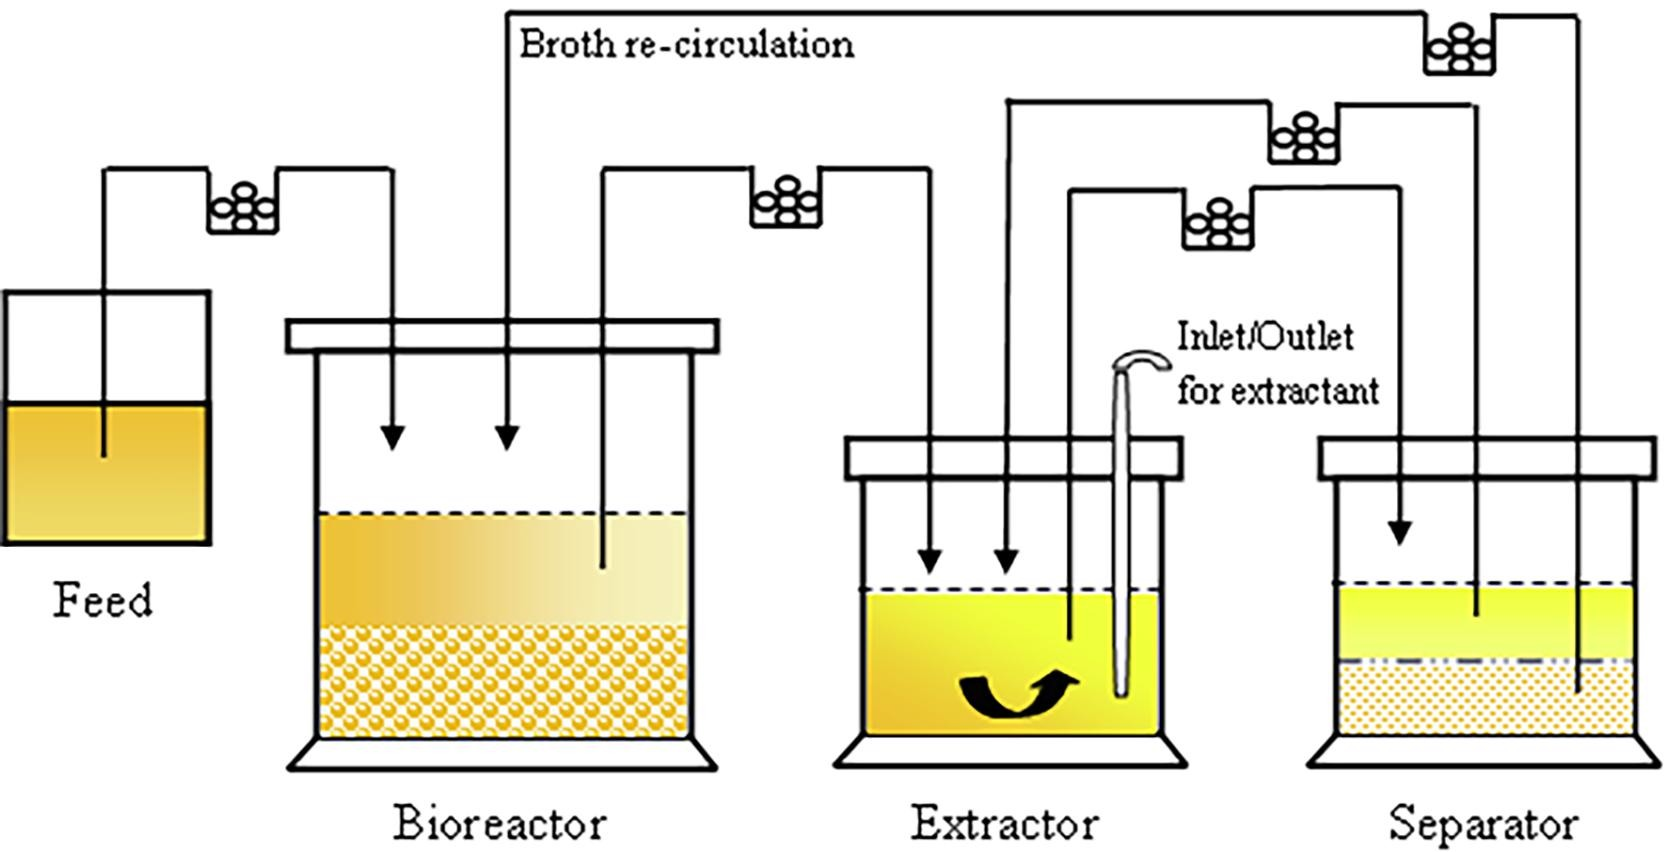
\includegraphics[width=9.5cm]{images/7.2.jpg}
                \captionsetup{font={small,bf,stretch=1.25}}%图注格式设置
                \caption{Sample picture}
                \label{fig1}%标签,该图引用格式  \ref{fig1}
            \end{figure}

            \begin{enumerate}
                \item[*] 条目一
                \item[*] 条目二
                \item[*] 条目三
            \end{enumerate}



\end{document}
\message{ !name(main.tex) !offset(-116) }
